\documentclass[12pt]{article}

\usepackage{sbc-template}
\usepackage{graphicx}
\usepackage[utf8]{inputenc}  
    
\sloppy

\title{Guia 3 - Introdução ao Logism}

\author{Luca Ribeiro Schettino Regne}

\address{Instituto de Ciências Exatas e Informática - ICEI - (PUC-MG)}

\begin{document} 

\maketitle

\section{Exercício 01}
\subsection{Circuito 1}
A + 0 = A\\\\
\\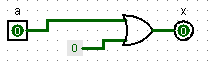
\includegraphics{./images/circuito01.png}\\
\\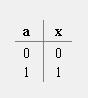
\includegraphics{./images/circuito01_table.png}

\subsection{Circuito 2}
A + 1 = 1\\
\\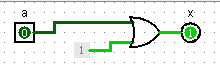
\includegraphics{./images/circuito02.png}\\
\\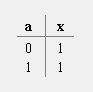
\includegraphics{./images/circuito02_table.png}

\subsection{Circuito 3}
A + A = A\\
\\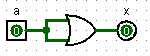
\includegraphics{./images/circuito03.png}\\
\\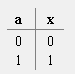
\includegraphics{./images/circuito03_table.png}

\subsection{Circuito 4}
~A + A = A\\
\\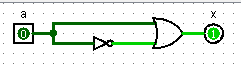
\includegraphics{./images/circuito04.png}\\
\\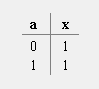
\includegraphics{./images/circuito04_table.png}

\subsection{Circuito 5}
A + AB = A\\
\\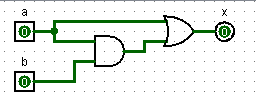
\includegraphics{./images/circuito05.png}\\
\\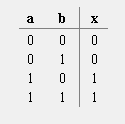
\includegraphics{./images/circuito05_table.png}

\subsection{Circuito 6}
A   B + A~B = A\\
\\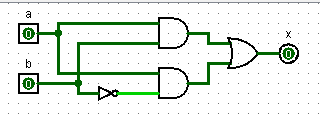
\includegraphics{./images/circuito06.png}\\
\\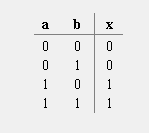
\includegraphics{./images/circuito06_table.png}

\subsection{Circuito 7}
A + ~AB = A ? B\\
\\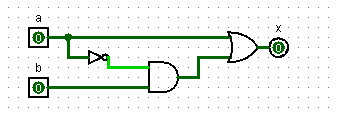
\includegraphics{./images/circuito07.png}\\
\\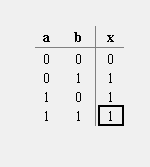
\includegraphics{./images/circuito07_table.png}

\subsection{Circuito 8}
A + BC = (A ? B)(A ? C)\\
\\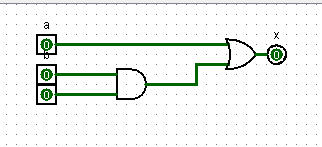
\includegraphics{./images/circuito08.png}\\
\\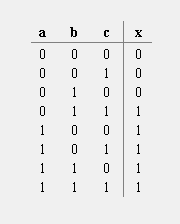
\includegraphics{./images/circuito08_table.png}

\section{Exercício 02}
\subsection{Circuito 01}
\\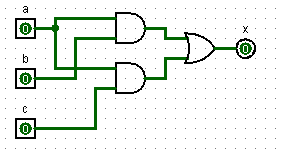
\includegraphics{./images/exercicio02_circuito01.png}
\\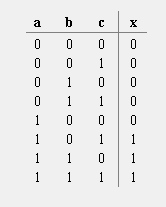
\includegraphics{./images/exercicio02_circuito01_table.png}

\subsection{Circuito 02}
\\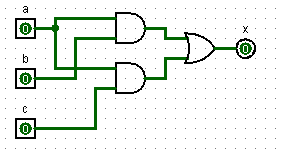
\includegraphics{./images/exercicio02_circuito01.png}
\\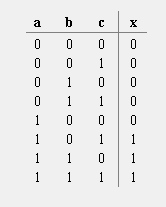
\includegraphics{./images/exercicio02_circuito01_table.png}

\section{Exercício 03}
A B = 0
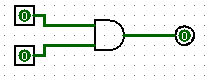
\includegraphics{./images/exercicio03_circuito.png}

\section{Exercício 04}
~(~(A B)) = 0
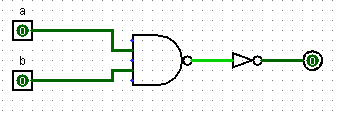
\includegraphics{./images/exercicio04_circuito.png}


\end{document}